In this section we will discuss  a number of issues pertaining to
linear algebra on parallel computers. We will take a realistic view of
this topic, assuming that the number of processors is finite, and that
the problem data is always large, relative to the number of
processors. We will also pay attention to the physical aspects of the
communication network between the processors. 

We will analyze various linear algebra operations, including iterative
methods, and their behaviour in the presence of a network with finite
bandwidth and finite connectivity. This chapter will conclude with
various short remarks regarding complications in algorithms that arise
due to parallel execution.

\Level 0 {Parallel dense matrix-vector product}
\label{sec:blockrow}
\index{Dense linear algebra|(}

In designing a parallel version of an algorithm, one often proceeds by
making a \indexterm {data decomposition} of the objects involved. In
the case of a matrix-vector operations such as the product $y=Ax$, we
have the choice of starting with a vector decomposition, and exploring
its ramifications on how the matrix can be decomposed, or rather to
start with the matrix, and deriving the vector decomposition from it.
In this case, it seems natural to start with decomposing the matrix
rather than the vector, since it will be most likely of larger
computational significance. We now have two choices:
\begin{enumerate}
\item We make a one-dimensional decomposition of the matrix, splitting
  it in block rows or block columns, and assigning each of these --~or
  groups of them~-- to a processor.
\item Alternatively, we can make a two-dimensional decomposition,
  assigning to each processor one or more general submatrices.
\end{enumerate}

We start by considering the decomposition in block rows. Consider
a processor~$p$ and the set $I_p$ of indices of rows that it
owns\footnote{For ease of exposition we will let $I_p$ be a contiguous
  range of indices, but any general subset is allowed.}, and
let $i\in I_p$ be a row that is assigned to this processor. 
%(In
%illustrations we will let $I_p$ be a consecutive set, but this need
%not be true in general.) 
The elements in
row~$i$ are used in the operation
\[ y_i=\sum_ja_{ij}x_j \]
We now reason:
\begin{itemize}
\item If processor $p$ has all $x_j$ values, the matrix-vector product
  can trivially be executed, and upon completion, the processor has
  the correct values~$y_j$ for~$j\in I_p$.
\item This means that every processor needs to have a copy of~$x$,
  which is wasteful. Also it raises the question of data integrity:
  you need to make sure that each processor has the correct value
  of~$x$.
\item In certain practical applications (for instance iterative
  methods, as you have seen before), the output of the matrix-vector
  product is, directly or indirectly, the input for a next
  matrix-vector operation. This is certainly the case for the power
  method which computes $x, Ax, A^2x,\ldots$. Since our operation
  started with each processor having the whole of~$x$, but ended with
  it owning only the local part of~$Ax$, we have a mismatch.
\item Maybe it is better to assume that each processor, at the start
  of the operation, has only the local part of~$x$, that is,
  those~$x_i$ where~$i\in I_p$, so that the start state and end state
  of the algorithm are the same. This means we have to change the
  algorithm to include some communication that allows each processor
  to obtain those values~$x_i$ where~$i\not\in\nobreak I_p$.
\end{itemize}

\begin{exercise}
  Go through a similar reasoning for the case where the matrix is
  decomposed in block columns. Describe the parallel algorithm in
  detail, like above, but without giving pseudo code.
\end{exercise}

\def\sublocal{_{\mathrm\scriptstyle local}}

Let us now look at the communication in detail: we will consider a
fixed processor~$p$ and consider the operations it performs and the
communication that necessitates.
According to the above analysis,
in executing the statement $y_i=\sum_ja_{ij}x_j$ we have
to be aware what processor the $j$ values `belong to'. To acknowledge
this, we write
\begin{equation}
  y_i=\sum_{j\in I_p}a_{ij}x_j+\sum_{j\not\in I_p}a_{ij}x_j
  \label{eq:yi=sum-in-and-not}
\end{equation}
If $j\in I_p$, the instruction $y_i \leftarrow y_i + a_{aij} x_j$
involves only quantities that are already local to
the processor.
Let us therefore concentrate on the case
$j\not\in I_p$.
It would be nice if we could just write the statement
\begin{verbatim}
y(i) = y(i) + a(i,j)*x(j)
\end{verbatim}
and some lower layer would automatically transfer \verb+x(j)+ from
whatever processor it is stored on to a local register. (The PGAS
languages of section~\ref{sec:pgas} aim to do this, but their
efficiency is far from guaranteed.) An implementation, based on this
optimistic view of parallelism, is given in figure~\ref{fig:naive-pmvp}.

\begin{figure}
  \begin{displayprocedure}{Naive Parallel MVP}{$A,x\sublocal,y\sublocal,p$}
    \KwIn{Processor number~$p$; the elements $x_i$ with $i\in I_p$; matrix
      elements $A_{ij}$ with $i\in I_p$.}
    \KwOut{The elements $y_i$ with $i\in I_p$}
    \For{$i\in I_p$}{$s\leftarrow0$\;
      \For{$j\in I_p$}{$s\leftarrow s+a_{ij}x_{j}$}
      \For{$j\not\in I_p$}{send $x_j$ from the processor that owns it to
        the current one, then\;  $s\leftarrow s+a_{ij}x_{j}$}
      $y_i\leftarrow s$
    }
  \end{displayprocedure}
  \caption{A na\"\i vely coded parallel matrix-vector product}
  \label{fig:naive-pmvp}
\end{figure}

The immediate problem with such a
`local' approach is that too much communication will take place.
\begin{itemize}
\item If the matrix $A$ is dense, the element $x_j$ is necessary once
  for each row $i\in I_p$, and it will thus be fetched once for every
  row~$i\in I_p$.
\item For each processor $q\not=p$, there will be (large) number of
  elements $x_j$ with $j\in I_q$ that need to be transferred from
  processor~$q$ to~$p$. Doing this in separate messages, rather than
  one bulk transfer, is very wasteful.
\end{itemize}
With shared memory these issues are not much of a problem, but in the
context of distributed memory it is better to take a
\indexterm{buffering} approach.

Instead of communicating individual elements of~$x$, we use a local
buffer $B_{pq}$ for each processor~$q\not=p$ where we collect the
elements from~$q$ that are needed to perform the product on~$p$. (See
\begin{figure}
  \begin{quote}
    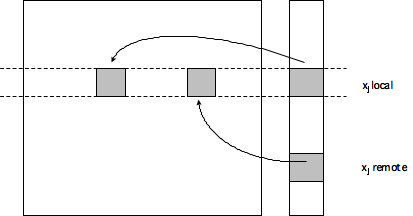
\includegraphics[scale=.12]{graphics/distmvp}
  \end{quote}
  \caption{The parallel matrix-vector product with a blockrow
    distribution.}
  \label{fig:distmvp2}
\end{figure}
figure~\ref{fig:distmvp2} for an illustration.) The parallel algorithm
is given in figure~\ref{fig:buffer-pmvp}.
\begin{figure}
\begin{displayprocedure}{Parallel MVP}{$A,x\sublocal,y\sublocal,p$}
  \KwIn{Processor number~$p$; the elements $x_i$ with $i\in I_p$; matrix
    elements $A_{ij}$ with $i\in I_p$.}
  \KwOut{The elements $y_i$ with $i\in I_p$}
  \For{$q\not=p$}{Send elements of~$x$ from processor $q$ to~$p$,
    receive in buffer~$B_{pq}$.}
  $y\sublocal\leftarrow A x\sublocal$\\
  \For{$q\not=p$}{$y\sublocal\leftarrow y\sublocal+A_{pq}B_q$}
\end{displayprocedure}
  \caption{A buffered implementation of the parallel matrix-vector
    product}
  \label{fig:buffer-pmvp}
\end{figure}

In addition to preventing an element from being fetched more than
once, this also combines many small messages into one large message,
which is usually more efficient; recall our discussion of bandwidth
and latency in section~\ref{sec:bwlatency}.

\begin{exercise}
  Give pseudocode for the matrix-vector product using 
  nonblocking operations (section~\ref{sec:nonblocking})
\end{exercise}

Above we said that having a copy of the whole of~$x$ on each processor
was wasteful in space. The implicit argument here is that, in general,
we do not want local storage to be function of the number of
processors: ideally it should be only a function of the local
data. (This is related to weak scaling; section~\ref{sec:scaling}.)

You see that, because of communication considerations, we have
actually decided that it is unavoidable, or at least preferable, for
each processor to store the whole input vector.  Such trade-offs
between space and time efficiency are fairly common in parallel
programming. For the dense matrix-vector product we can actually
defend this overhead, since the vector storage is of lower order than
the matrix storage, so our over-allocation is small by ratio. Below
(section~\ref{sec:pspmvp}), we will see that for the sparse
matrix-vector product the overhead can be much less.

It is easy to see that the parallel dense matrix-vector product, as
described above, has perfect speedup \emph{if we are allowed to ignore
  the time for communication}. In the next section you will see that
the block row implementation above is not optimal if we take
communication into account. For scalability
we need a two-dimensional decomposition.

\Level 0 {Scalability of the dense matrix-vector product}
\label{sec:densescaling}

\input chapters-public/mvpscaling2

\Level 0 {Scalability of LU factorization}
\label{sec:LUscaling}

A full analysis of the scalability of dense LU factorization is quite
involved, so we will state without further proof that again a
two-dimensional distribution is needed. However, we can identify a
further complication. Since factorizations of any
type\footnote{Gaussian elimination can be performed in right-looking,
  left-looking and Crout variants; see~\cite{TSoPMC}.}
progress through a matrix, processors will be inactive for part of the
time.

\begin{exercise}
  Consider the regular right-looking Gaussian elimination
\begin{verbatim}
for k=1..n
  p = 1/a(k,k)
  for i=k+1,n
    for j=k+1,n
      a(i,j) = a(i,j)-a(i,k)*p*a(k,j)
\end{verbatim}
  Analyze the running time, speedup, and efficiency as a function
  of~$N$, if we assume a one-dimensional distribution, and enough
  processors to store one column per processor. Show that speedup is
  limited.

  Also perform this analysis for a two-dimensional decomposition where
  each processor stores one element.
\end{exercise}

\index{matrix!storage, dense|(}

For this reason, an \indexterm{overdecomposition} is used, where
the matrix is divided in more blocks than there are processors,
and each processor stores several, non-contiguous, sub-matrices. 
\begin{figure}[ht]
  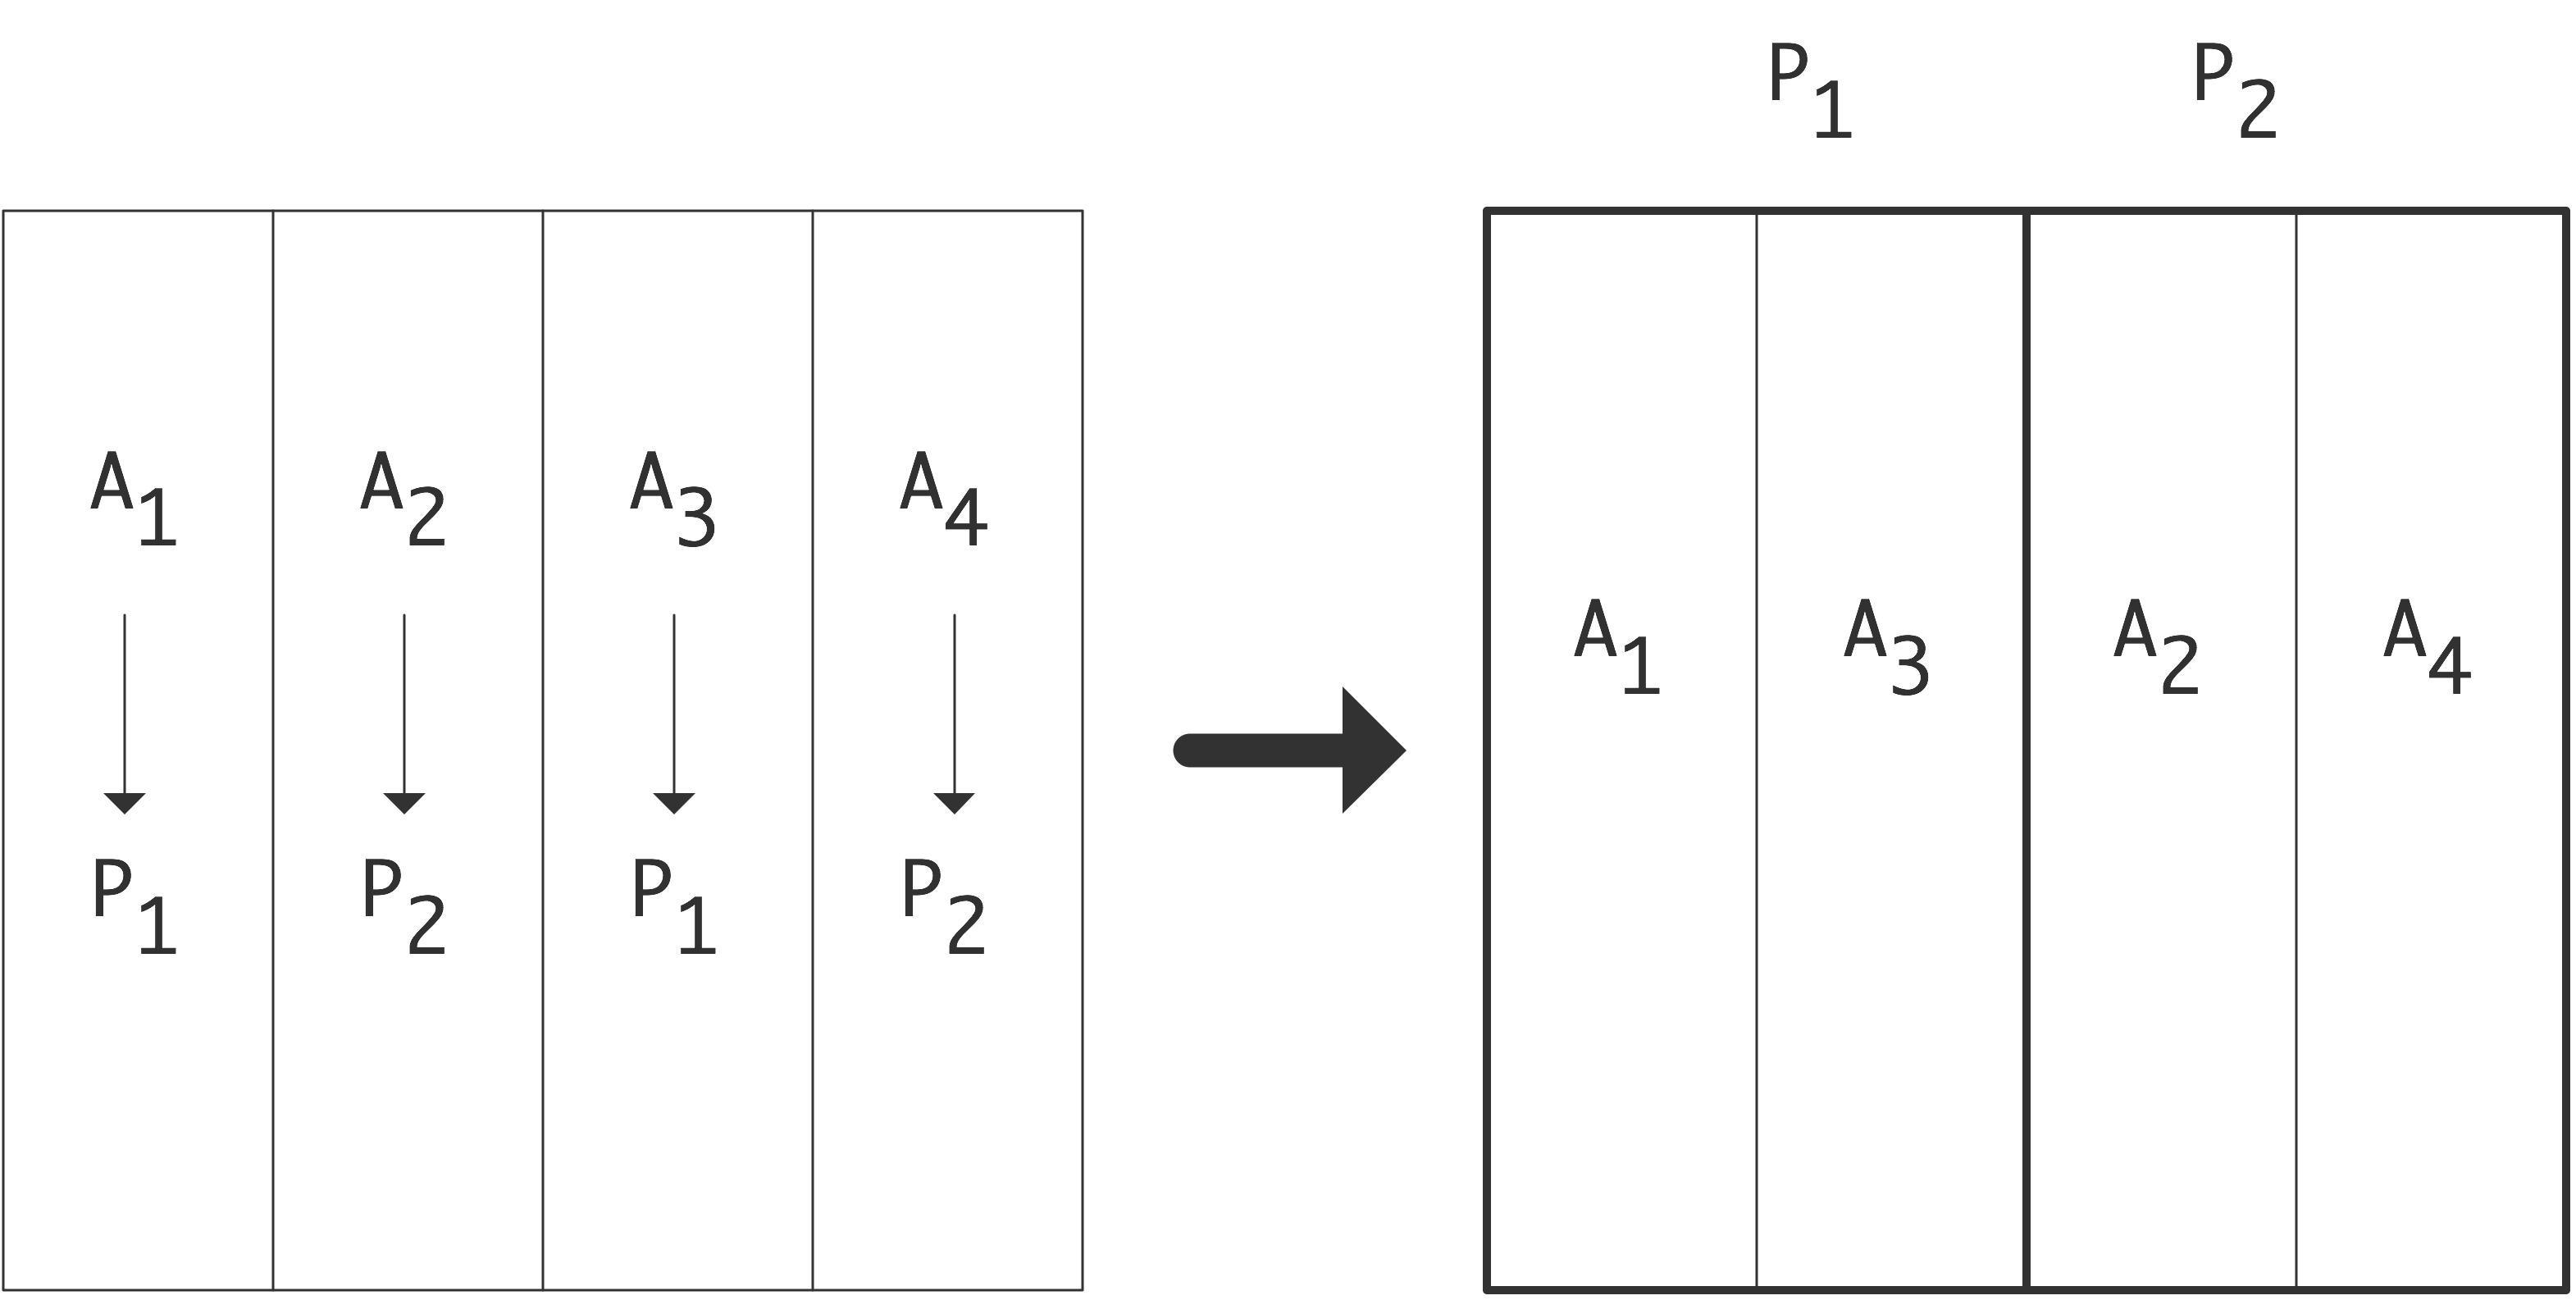
\includegraphics[scale=.11]{graphics/cyclic-1}
  \caption{One-dimensional cyclic distribution: assignment of four
    matrix columns to two processors, and the resulting mapping of
    storage to matrixcolumns}
  \label{fig:cyclic-1}
\end{figure}
We illustrate this in figure~\ref{fig:cyclic-1} where we divide four
block columns of a matrix to two processors: each processor stores in
a contiguous block of memory two non-contiguous matrix columns.

Next, we illustrate in figure~\ref{fig:cyclic-1-mvp}
\begin{figure}[ht]
  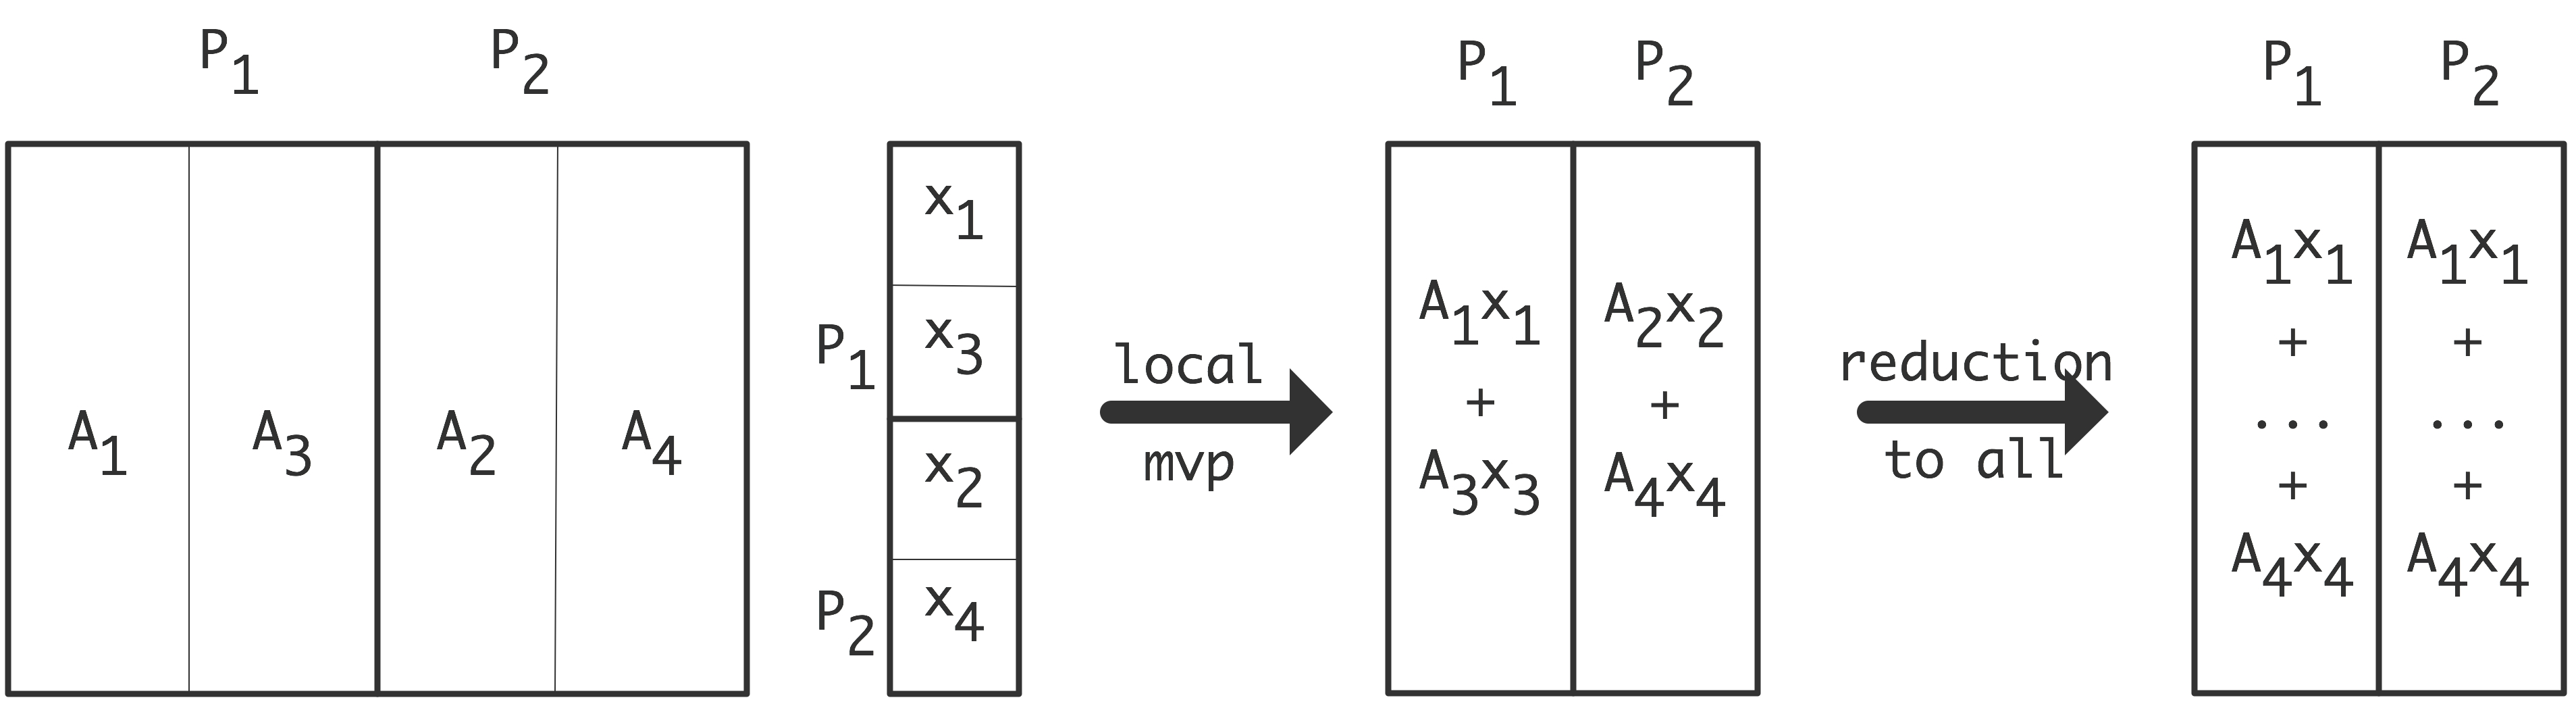
\includegraphics[scale=.11]{graphics/cyclic-1-mvp}
  \caption{Matrix-vector multiplication with a cyclicly distributed matrix}
  \label{fig:cyclic-1-mvp}
\end{figure}
that a matrix-vector product with such a matrix can be performed
without knowing that the processors store non-contiguous parts of the
matrix. All that is needed is that the input vector is also cyclicly
distributed.

\begin{exercise}
  Now consider a $4\times4$ matrix and a $2\times2$ processor
  grid. Distribute the matrix cyclicly both by rows and columns. Show
  how the matrix-vector product can again be performed using the
  contiguous matrix storage, as long as the input is distributed
  correctly. How is the output distributed? Show that more
  communication is needed than the reduction of the one-dimensional
  example.
\end{exercise}

Specifically,
with $P<N$ processors, and assuming for simplicity $N=cP$, we let
processor~0 store rows $0,c,2c,3c,\ldots$; processor~1 stores rows
$1,c+1,2c+1,\ldots$, et cetera. This scheme can be generalized two a
two-dimensional distribution, if $N=c_1P_1=c_2P_2$
and~$P=P_1P_2$. This is called a 2D \indexterm{cyclic
  distribution}. This scheme can be further extended by considering
block rows and colums (with a small block size), and assigning to
processor~0 the \emph{block} rows $0,c,2c,\ldots$.

\begin{exercise}
  Consider a square $n\times n$ matrix, and a square $p\times p$
  processor grid, where $p$ divides~$n$ without remainder. Consider
  the overdecomposition outlined above, and make a sketch of matrix
  element assignment for the specific case $n=6,p=2$. That is, draw an
  $n\times n$ table where location $(i,j)$ contains the processor
  number that stores the corresponding matrix element. Also make a
  table for each of the processors describing the local to global mapping,
  that is, giving the global $(i,j)$ coordinates of the elements in
  the local matrix. (You will find this task facilitated by using
  zero-based numbering.)

  Now write functions $P,Q,I,J$ of $i,j$ that describe the global to
  local mapping, that is, matrix element $a_{ij}$ is stored in
  location $(I(i,j),J(i,j))$ on processor $(P(i,j),Q(i,j))$.
\end{exercise}

\index{matrix!storage, dense|)}

\index{Dense linear algebra|)}

\Level 0 {Parallel sparse matrix-vector product}
\label{sec:pspmvp}
\index{sparse!linear algebra|(}
\input chapters-public/spmvp
\index{sparse!linear algebra|)}

\Level 0 {Computational aspects of iterative methods}
\label{sec:iterative-computational}

All iterative methods feature the following operations:
\begin{itemize}
\item A matrix-vector product; this was discussed for the sequential
  case in section~\ref{sec:sparse} and for the parallel case in
  section~\ref{sec:pspmvp}.
  In the parallel case,
  construction of \ac{FEM} matrices has a complication that we will
  discuss in section~\ref{sec:fem-assembly}.
\item The construction of the preconditioner matrix~$K\approx A$, and
  the solution of systems $Kx=y$. This was discussed in the sequential
  case in section~\ref{sec:preconditioner}. Below
  we will go into parallelism aspects in section~\ref{sec:parallel-prec}.
\item Some vector operations (including inner products, in
  general). These will be discussed next.
\end{itemize}

\Level 1 {Vector operations}

There are two types of vector operations in a typical iterative method:
vector additions and inner products. 

\begin{exercise}
  Consider the \ac{CG} method of section~\ref{sec:cg},
  figure~\ref{fig:pcg}, applied to the
  matrix from a 2D \ac{BVP}; equation~\eqref{eq:5starmatrix}, First
  consider the unpreconditioned case $M=I$. Show that there is a
  roughly equal number of floating point
  operations are performed in the matrix-vector product and 
  in the vector operations. Express everything in the matrix size~$N$ and
  ignore lower order terms. How would this balance be if the matrix
  had 20 nonzeros per row?

  Next, investigate this balance between vector and matrix operations
  for the \ac{FOM} scheme in section~\ref{sec:fom}. Since the number
  of vector operations depends on the iteration, consider the first 50
  iterations and count how many floating point operations are done in
  the vector updates and inner product versus the matrix-vector
  product. How many nonzeros does the matrix need to have for these
  quantities to be equal?
\end{exercise}

\begin{exercise}
  Flop counting is not the whole truth. What can you say about the
  efficiency of the vector and matrix operations in an iterative
  method, executed on a single processor?
\end{exercise}

\Level 2 {Vector additions}

The vector additions are
typically of the form $x\leftarrow x+\alpha y$ or $x\leftarrow \alpha x+y$.
If we assume that all vectors are distributed the same way, this
operation is fully parallel.

\Level 2 {Inner products}
\index{inner products|(}

Inner products are vector operations, but they are computationally
more interesting than updates, since they involve communication. 

When we compute an inner product, most likely 
every processor needs to receive the computed value. We
use the following algorithm:

\begin{displayalgorithm}
  \For {processor $p$} {
    compute $a_p\leftarrow x_p^ty_p$ where $x_p,y_p$ are the part of
    $x,y$ stored on processor~$p$ }
    do a global reduction to compute $a=\sum_p a_p$ \;
    broadcast the result
  \caption{Compute $a\leftarrow x^ty$ where $x,y$ are distributed vectors}
\end{displayalgorithm}

The reduction and broadcast (which can be joined into an {\tt
  Allreduce}) combine data over all processors, so they have a
communication time that increases with the number of processors. This
makes the inner product potentially an expensive operation, and people
have suggested a number of ways to reducing their impact on the
performance of iterative methods.

\begin{exercise}
  Iterative methods are typically used for sparse matrices. In that
  context, you can argue that the communication involved in an inner product
  can have a larger influence on overall performance than the
  communication in the matrix-vector product. What is the
  complexity of the matrix-vector product and the inner product as a
  function of the number of processors?
\end{exercise}

Here are some of the approaches that have been taken.
\begin{itemize}
\item The \ac{CG} method has two inner products per iteration that are
  inter-dependent. It is possible to rewrite the method so that it
  computes the same iterates (in exact arithmetic, at least) but so
  that the two inner products per iteration can be
  combined. See~\cite{ChGe:sstep,DAzEijRo:ppscicomp,Me:multicg,YandBrent:bicgstab}.
\item It may be possible to overlap the inner product calculation with
  other, parallel, calculations~\cite{dehevo92:acta}.
\item In the \ac{GMRES} method, use of the classical \acf{GS}
  method takes far fewer independent inner product than the modified
  \ac{GS} method, but it is less stable. People have investigated strategies for deciding
  when it is allowed to use the classic \ac{GS} method~\cite{Langou:thesis}.
\end{itemize}

\index{inner products|)}

\Level 1 {Finite element matrix construction}
\label{sec:fem-assembly}

The \indexac{FEM} leads to an interesting issue in parallel
computing. For this we need to sketch the basic outline of how this
method works. The \ac{FEM} derives its name from the fact that the
physical objects modeled are divided into small two or three
dimensional shapes, the elements, such as triangles and squares in 2D,
or pyramids and bricks in~3D. On each of these, the function we are
modeling is then assumed to polynomial, often of a low degree, such as
linear or bilinear.

\begin{figure}[ht]
  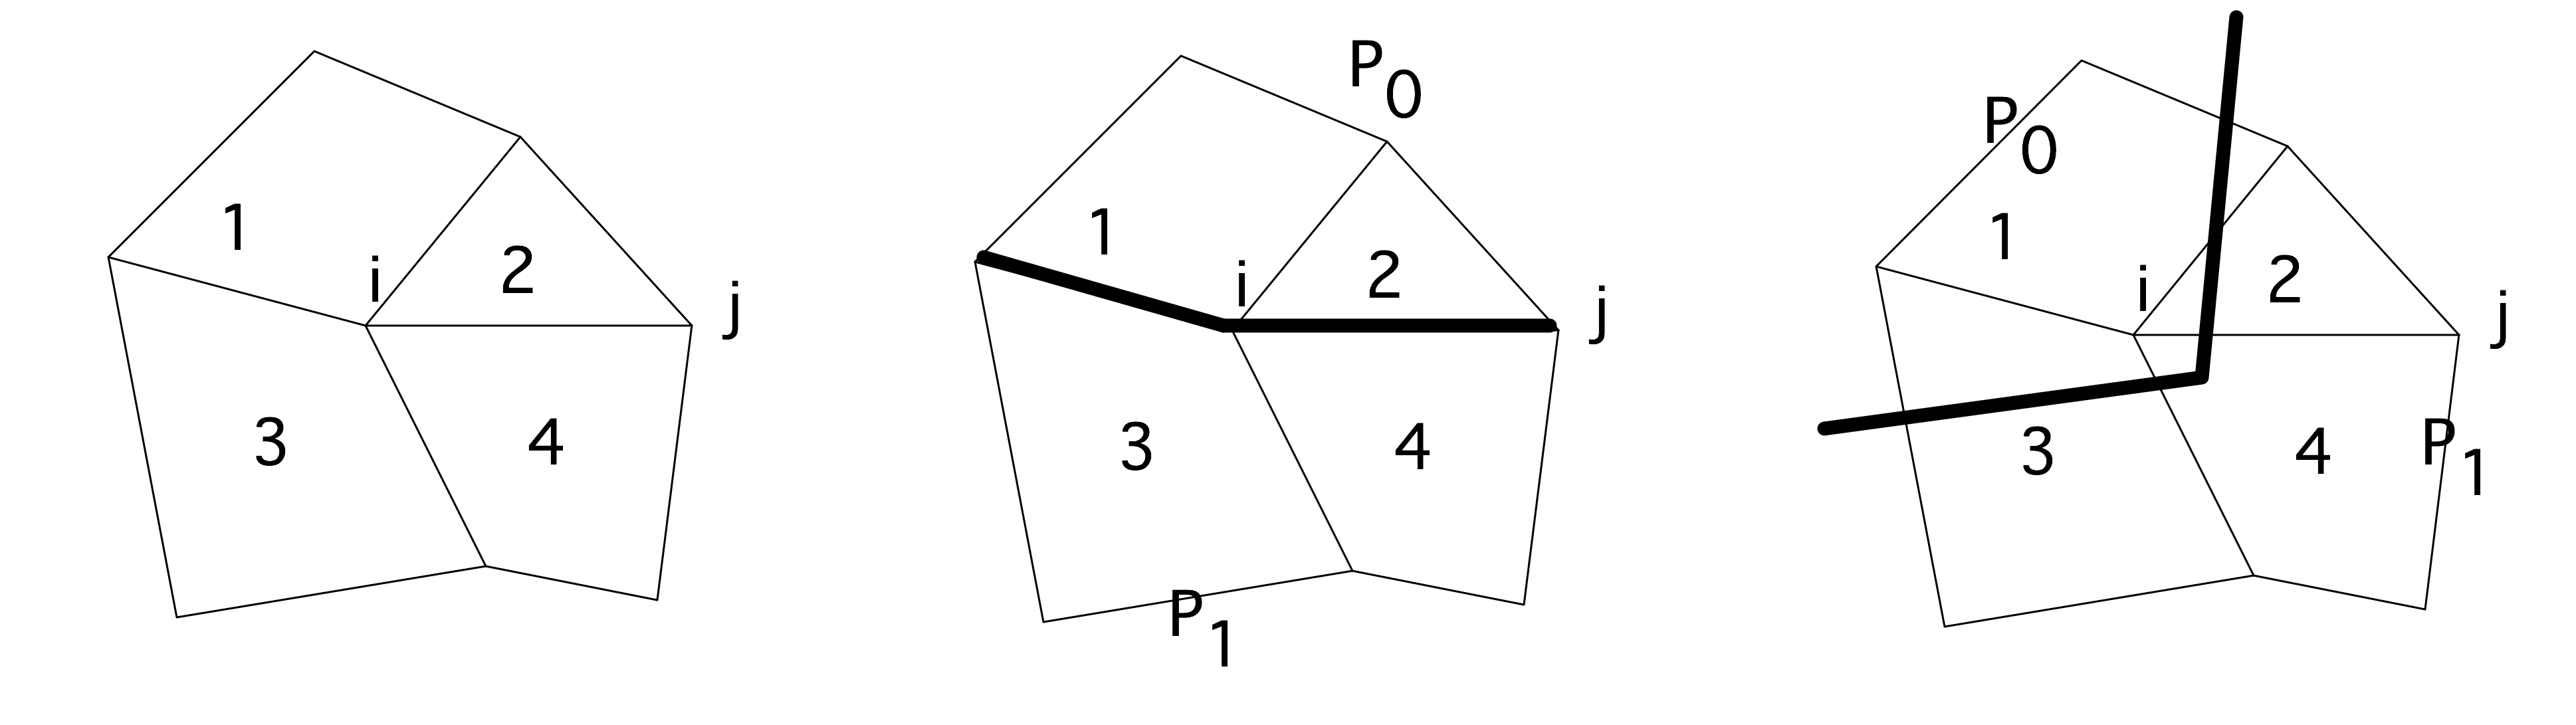
\includegraphics[scale=.12]{graphics/fem}  
  \caption{A finite element domain, parallelization of the matrix
    construction, and parallelization of matrix element storage}
  \label{fig:fem-assembly}
\end{figure}

The crucial fact is that a matrix element~$a_{ij}$ is then the sum of
computations, specifically certain integrals, over all elements that
contain both variables $i$ and~$j$:
\[ a_{ij}=\sum_{e\colon i,j\in e} a^{(e)}_{ij}. \]
The computations in each element share many common parts, so it is
natural to assign each element~$e$ uniquely to a processor~$P_e$,
which then computes all contributions~$a^{(e)}_{ij}$. In
figure~\ref{fig:fem-assembly} element~2 is assigned to processor~0
and element~4 to processor~1.

Now consider variables $i$ and~$j$ and the matrix
element~$a_{ij}$.  It is constructed as the sum of computations over
domain elements 2 and~4, which have been assigned to different processors.
Therefore, no matter what processor row $i$ is assigned to, at least
one processor will have to communicate its contribution to matrix
element~$a_{ij}$.

Clearly it is not possibly to make assignments $P_e$ of elements and
$P_i$ of variables such that $P_e$ computes in full the coefficients
$a_{ij}$ for all $i\in e$. In other words, if we compute the
contributions locally, there needs to be some amount of communication to
assemble certain matrix elements.
For this reason, modern linear algebra libraries such as PETSc (see
tutorial section~\ref{tut:petsc}) allow any processor to set any
matrix element.

\Level 0 {Parallel preconditioners}
\label{sec:parallel-prec}

Above (sections \ref{sec:preconditioner} and \ref{sec:ilu}) we saw a
couple of different choices of~$K$. In this section we will begin the
discussion of parallelization strategies. The discussion is continued
in detail in the next sections.

\Level 1 {Jacobi preconditioning}

The Jacobi method (section~\ref{sec:jacobi-seidel}) uses the diagonal
of~$A$ as preconditioner. Applying this is as parallel as is
possible: the statement $y\leftarrow K\inv x$ scales every element of
the input vector independently. Unfortunately the improvement in the
number of iterations with a Jacobi preconditioner is rather
limited. Therefore we need to consider more sophisticated methods such
\ac{ILU}. Unlike with the Jacobi preconditioner, parallelism is then
not trivial.

\Level 1 {The trouble with parallel ILU}

Above we saw that, in a flop counting sense, applying an ILU
preconditioner (section~\ref{sec:ilu}) is about as expensive as doing
a matrix-vector product. This is no longer true if we run our
iterative methods on a parallel computer.

At first glance the operations are similar. A matrix-vector product
$y=Ax$ looks like
\begin{verbatim}
for i=1..n
  y[i] = sum over j=1..n a[i,j]*x[j]
\end{verbatim}
In parallel this would look like
\begin{verbatim}
for i=myfirstrow..mylastrow
  y[i] = sum over j=1..n a[i,j]*x[j]
\end{verbatim}
Suppose that a processor has local copies of all the elements of $A$
and~$x$ that it will need, then this operation is fully parallel: each
processor can immediately start working, and if the work load is
roughly equal, they will all finish at the same time. The total time
for the matrix-vector product is then divided by the number of
processors, making the speedup more or less perfect.

Consider now the forward solve $Lx=y$, for instance in the context of
an \ac{ILU} preconditioner:
\begin{verbatim}
for i=1..n
  x[i] = (y[i] - sum over j=1..i-1 ell[i,j]*x[j]) / a[i,i]
\end{verbatim}
We can simply write the parallel code:
\begin{verbatim}
for i=myfirstrow..mylastrow
  x[i] = (y[i] - sum over j=1..i-1 ell[i,j]*x[j]) / a[i,i]
\end{verbatim}
but now there is a problem. We can no longer say `suppose a processor
has local copies of everything in the right hand side', since the
vector~$x$ appears both in the left and right hand side. While the
matrix-vector product is in principle fully parallel over the matrix
rows, this triangular solve code is recursive, hence sequential.

In a parallel computing context this means that, for the second
processor to start, it needs to wait for certain components of~$x$
that the first processor computes. Apparently, the second processor
can not start until the first one is finished, the third processor has
to wait for the second, and so on. The disappointing conclusion is
that in parallel only one processor will be active at any time, and
the total time is the same as for the sequential algorithm. This is
actually not a big problem in the dense matrix case, since parallelism
can be found in the operations for handling a single row (see
section~\ref{sec:multicore-block}), but in the sparse case it means we
can not use incomplete factorizations without some redesign.

In the next few subsections we will see different strategies for
finding preconditioners that perform efficiently in parallel.

\Level 1 {Block Jacobi methods}
\label{sec:block-jacobi}
\index{block Jacobi|(}

Various approaches have been suggested to remedy this sequentiality
the triangular solve. For instance, we could simply let the processors
ignore the components of~$x$ that should come from other processors:
\begin{verbatim}
for i=myfirstrow..mylastrow
  x[i] = (y[i] - sum over j=myfirstrow..i-1 ell[i,j]*x[j]) 
         / a[i,i]
\end{verbatim}
This is not mathematically equivalent to the sequential algorithm
(technically, it is called a \indexterm{block Jacobi} method with 
\ac{ILU} as the \indexterm{local solve}), but
since we're only looking for an approximationg $K\approx A$, this is
simply a slightly cruder approximation.
\begin{exercise}
  Take the Gauss-Seidel code you wrote above, and simulate a parallel
  run. What is the effect of increasing the (simulated) number of processors?
\end{exercise}

The idea behind block methods can easily be appreciated pictorially;
see figure~\ref{fig:block-method}.
\begin{figure}[ht]
  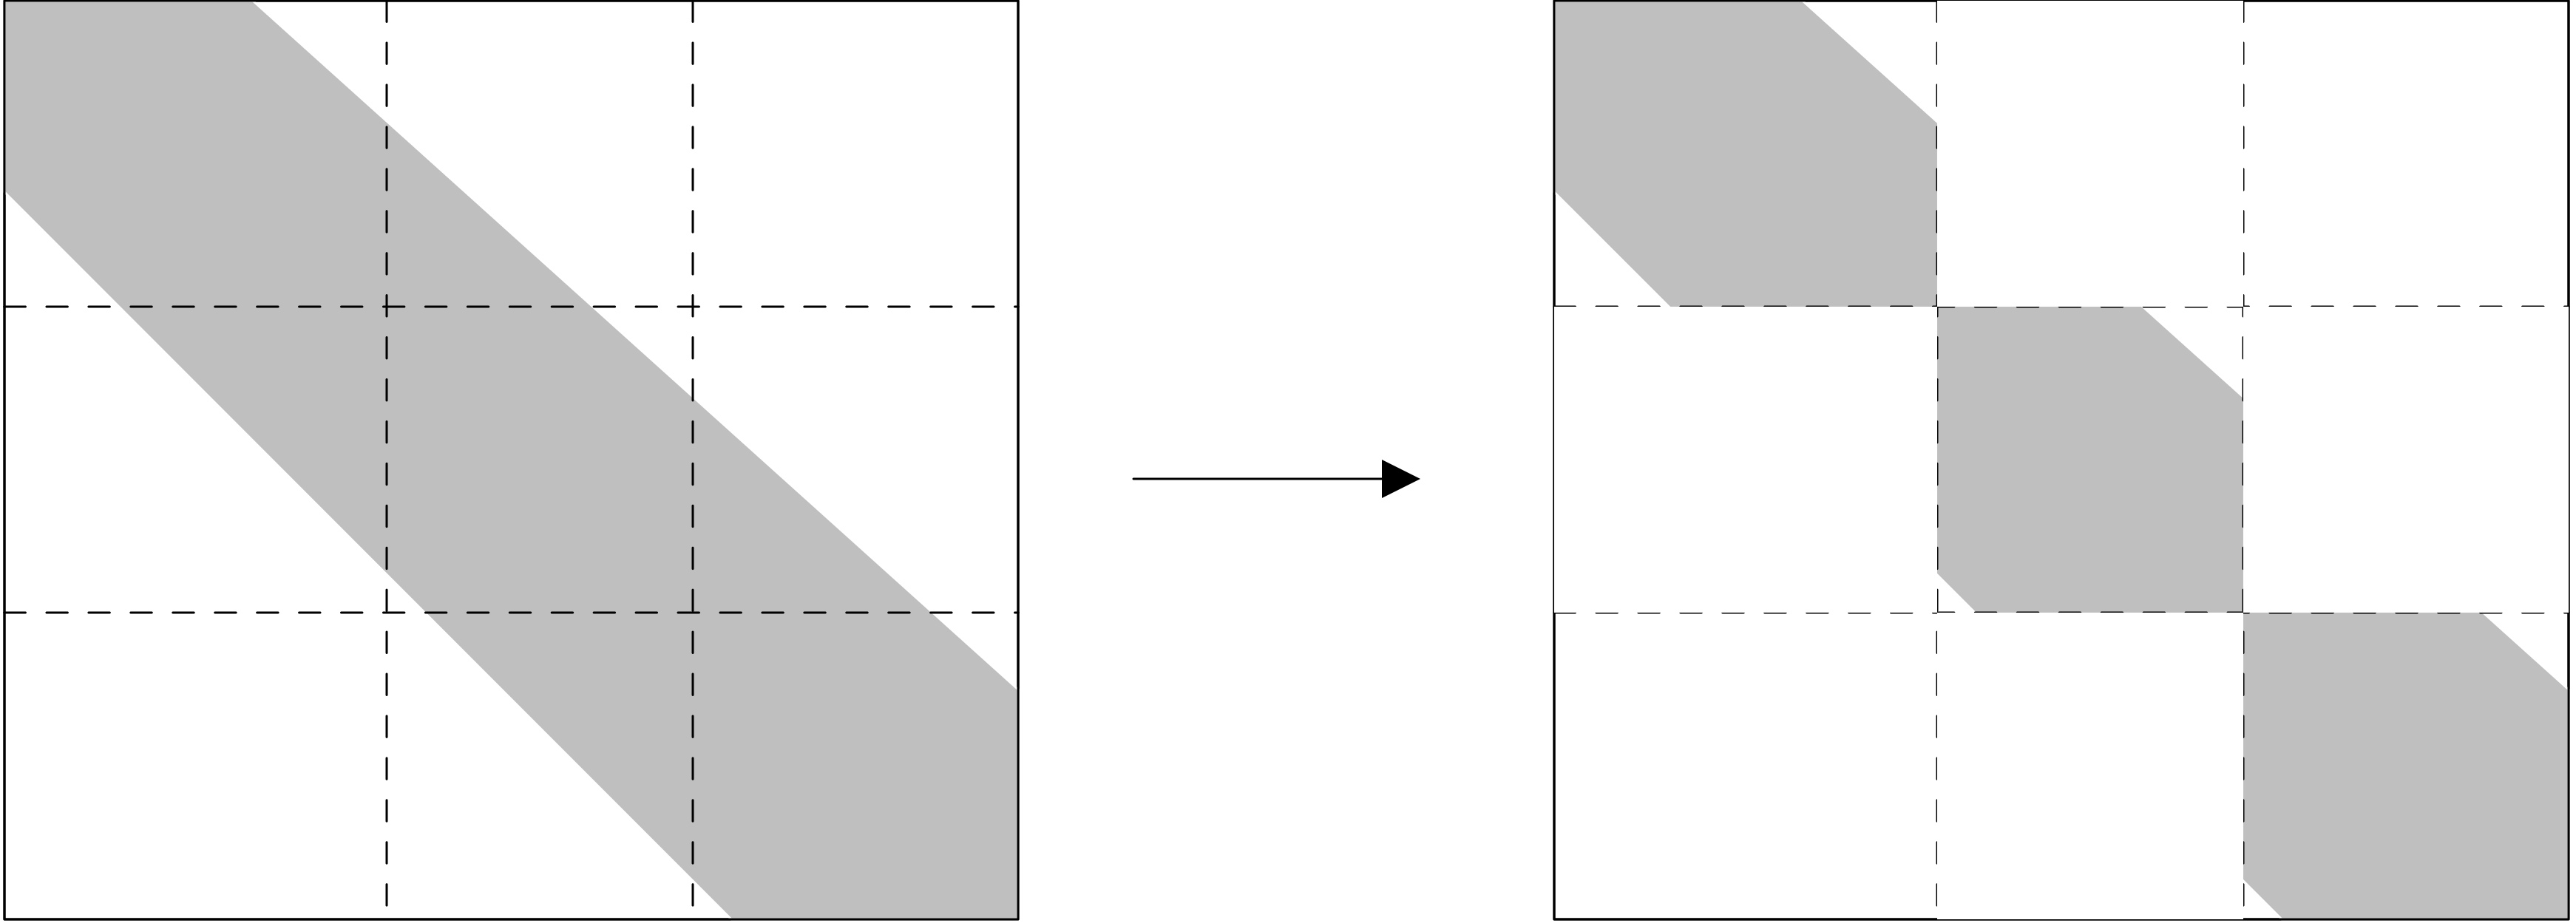
\includegraphics[scale=.12]{graphics/block-jacobi}
  \caption{Sparsity pattern corresponding to a block Jacobi
    preconditioner}
  \label{fig:block-method}
\end{figure}
In effect, we make an \ac{ILU} of the matrix that we get by ignoring
all connections between processors. Since in a \ac{BVP} all points
influence each other (see section~\ref{sec:region-influence}), using a
less connected preconditioner will increase the number of iterations
if executed on a sequential computer. However, block methods are
parallel and, as we observed above, a sequential preconditioner is
very inefficient in a parallel context, so we put up with this
increase in iterations.

\index{block Jacobi|)}

\Level 1 {Parallel ILU}
\label{sec:parallel-ilu}
\index{Incomplete LU (ILU)!parallel|(}

The Block Jacobi preconditioner operates by decoupling domain
parts. While this may give a method that is highly parallel, it may
give a higher number of iterations than a true \ac{ILU}
preconditioner. (A~theoretical argument can be made that this
decoupling decreases the efficiency of the iterative method; see
section~\ref{sec:region-influence}.) Fortunately it is possible to
have a parallel \ac{ILU} method.

In section~\ref{sec:redblackgreen} you saw the combination of
\indextermbus{graph}{colouring} and permutation. Let $P$ be the
permutation that groups like-coloured variables together, then $\tilde
A=P^tAP$ is a matrix with the following structure:
\begin{itemize}
\item $\tilde A$ has a block structure with the number of blocks equal
  to the number of colours in the adjacency graph of~$A$; and
\item each diagonal block is a diagonal matrix.
\end{itemize}
Now, if you are performing an iterative system solution
and you are looking for a parallel preconitioner you can use this
permuted matrix. Consider solving $Ly=x$ with the permuted system. We
write the usual algorithm (section~\ref{sec:lu-solve}) as
\begin{quotation}
  \begin{tabbing}
    for \=$c$ in the set of colours:\\
    \>for \=$i$ in the variables of colour $c$:\\
    \>\>$y_i\leftarrow x_i-\sum_{j<i} \ell_{ij}y_j$
  \end{tabbing}
\end{quotation}

\begin{exercise}
  Show that the flop count of solving a system $LUx=y$ remains the
  same (in the highest order term) when you from an \ac{ILU}
  factorization in the natural ordering to one in the colour-permuted
  ordering.
\end{exercise}

\begin{figure}
  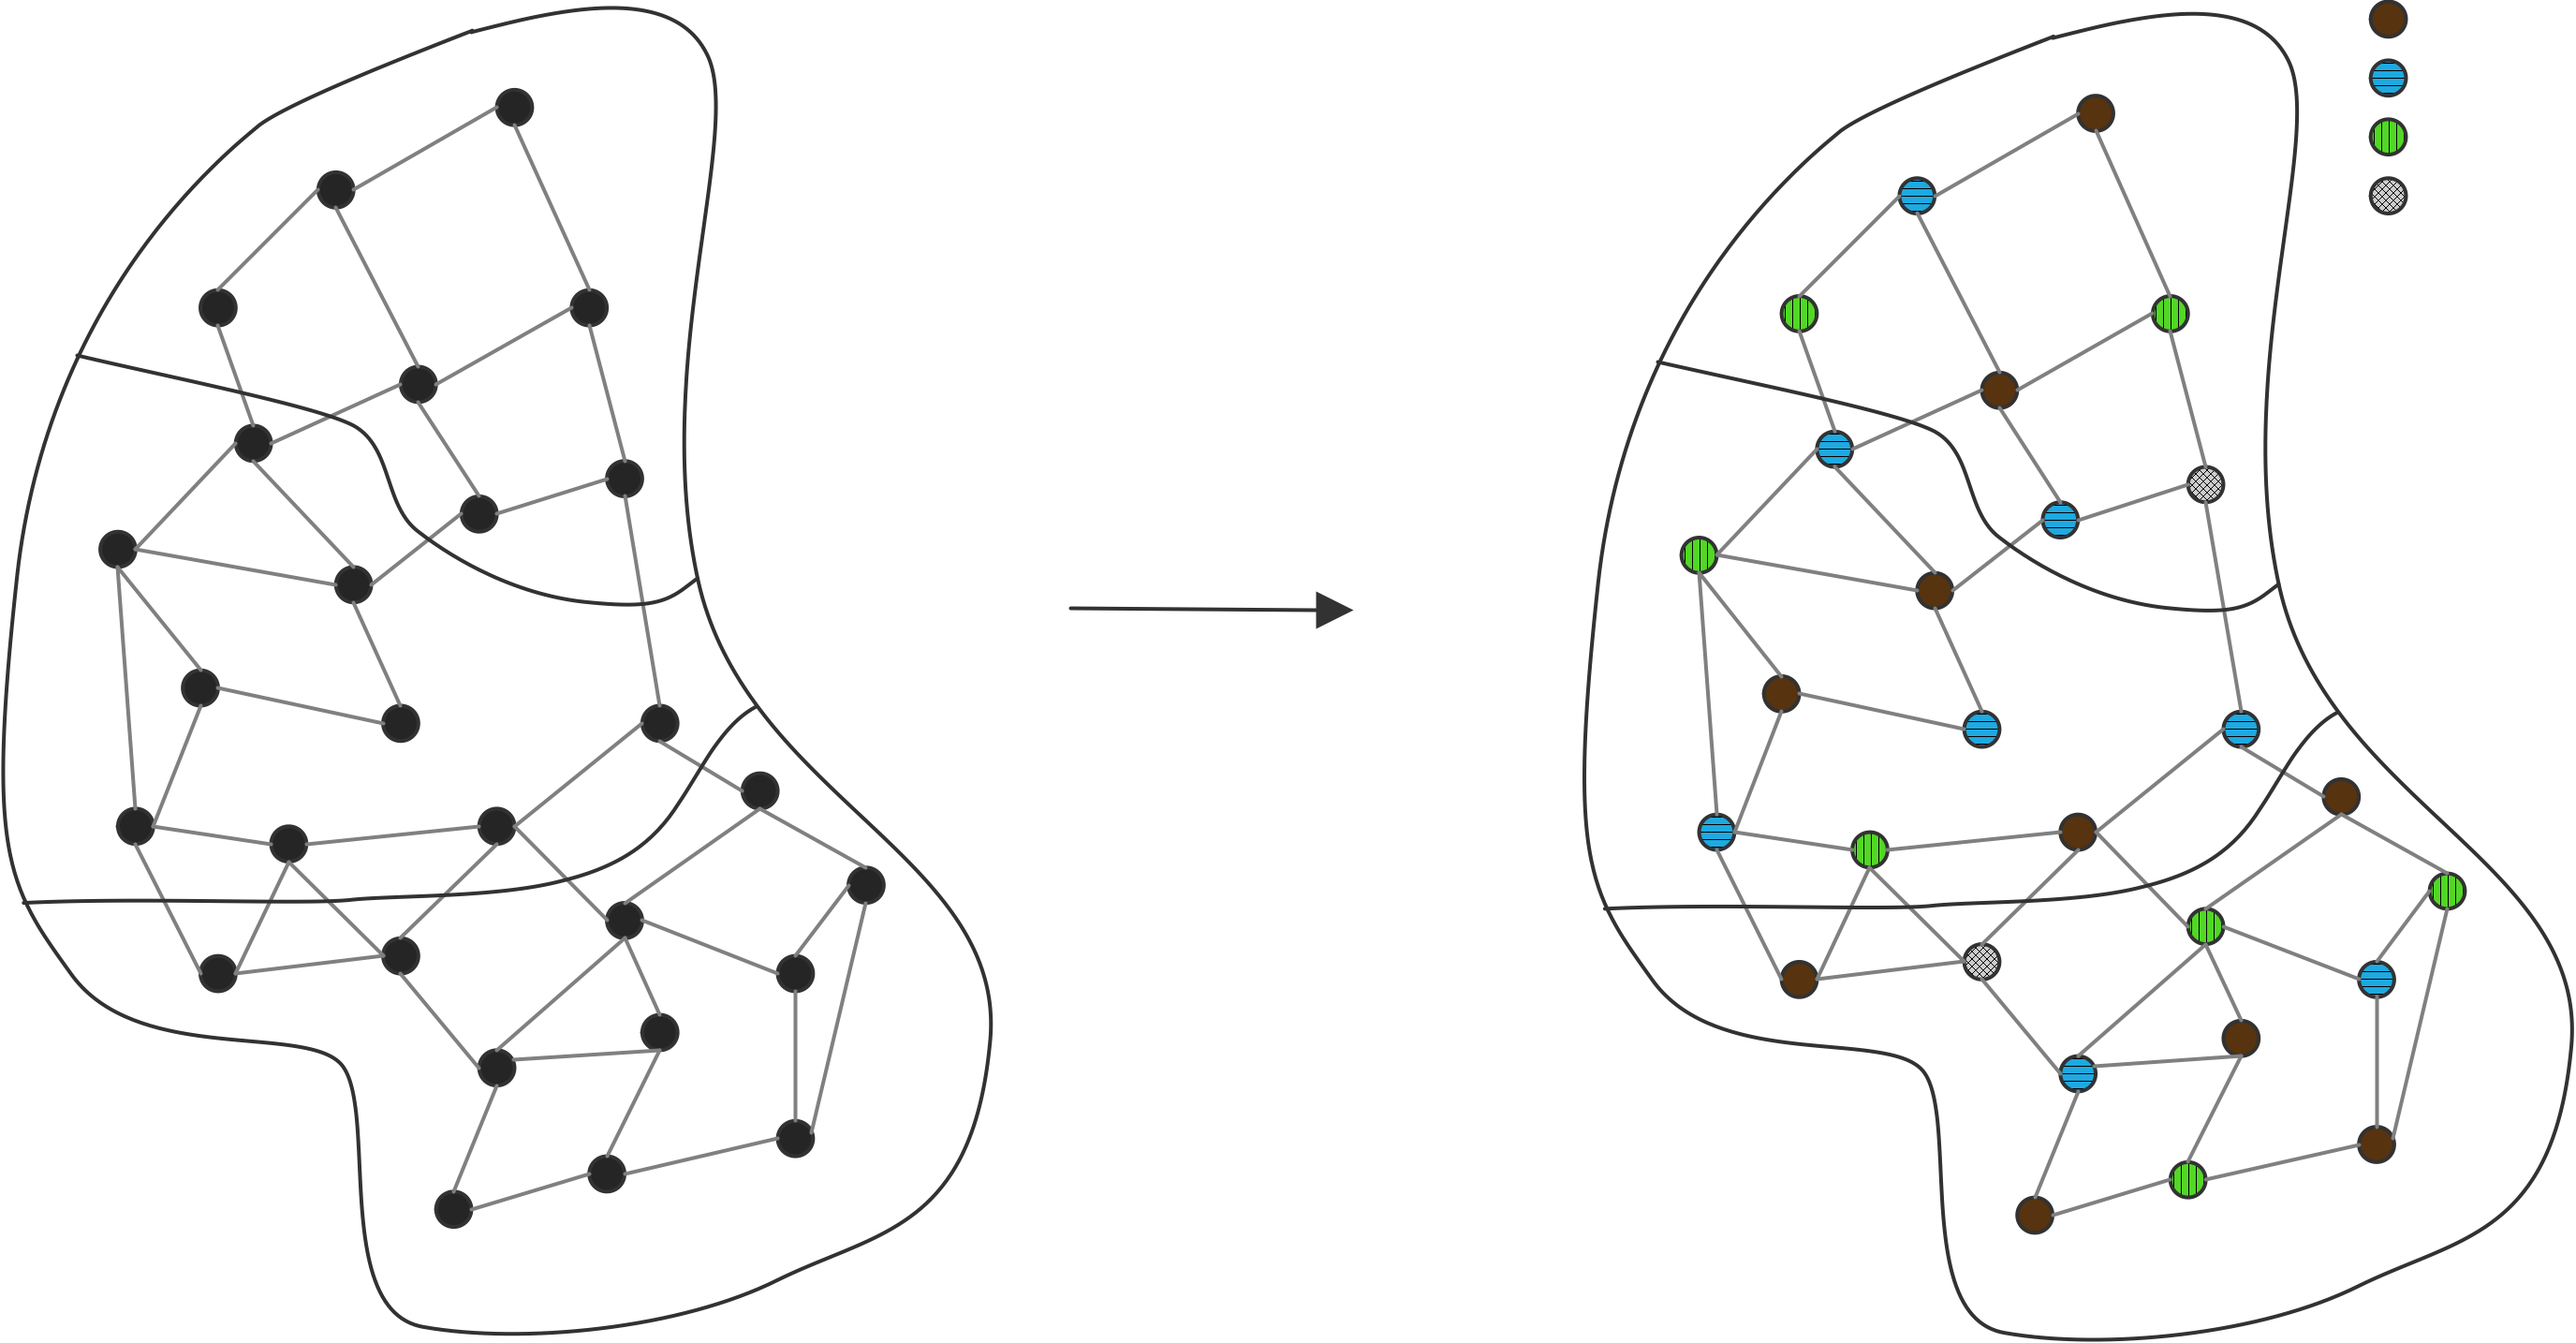
\includegraphics[scale=.1]{graphics/pilu}
  \caption{A partitioned domain with coloured nodes}
  \label{fig:pilu}
\end{figure}
Where does all this colouring get us? Solving is still
sequential\ldots Well, it is true that the outer loop over the colours
is sequential, but all the points of one colour are independent of
each other, so they can be solved at the same time.
\begin{figure}
  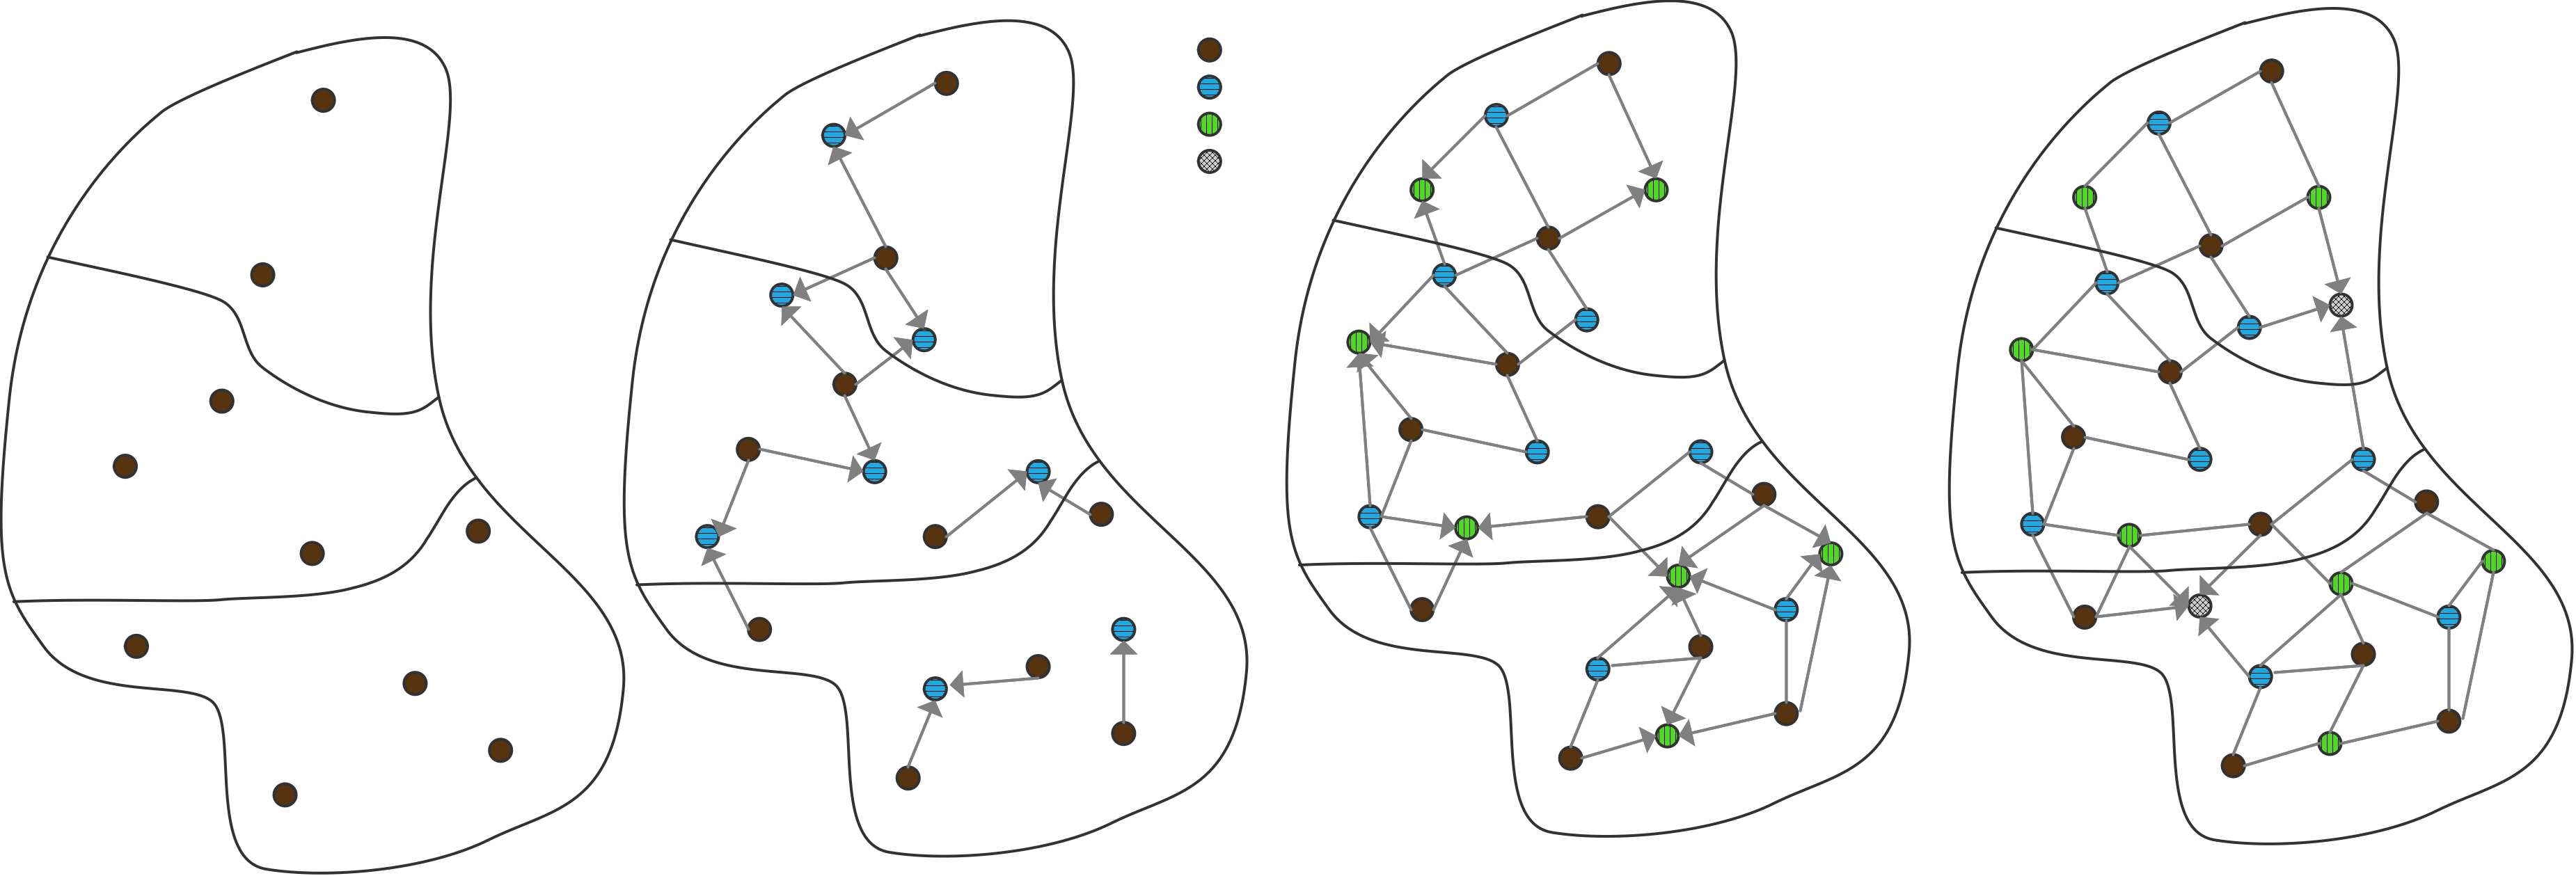
\includegraphics[scale=.12]{graphics/pilu-solve}
  \caption{Solving a parallel multicolour ILU in four steps}
  \label{fig:pilu-solve}
\end{figure}
So if we use an ordinary domain partitioning and combine that with a
multi-colouring (see figure~\ref{fig:pilu}), the processors are all
active during all the colour stages; see
figure~\ref{fig:pilu-solve}. Ok, if you take a close look at that
figure you'll see that one processor is not active in the last
colour. With large numbers of nodes per processor this is unlikely to
happen, but there may be some load inbalance.

\index{Incomplete LU (ILU)!parallel|)}

\Level 0 {Ordering strategies and parallelism}
\label{sec:ordering}

\Level 1 {Nested dissection}
\label{sec:dissection}
\index{nested dissection|(}
\input chapters-public/dissection
\index{nested dissection|)}
\Level 1 {Variable reordering and colouring: independent sets}
\label{sec:redblackgreen}
\input chapters-public/redblackgreen

\Level 0 {Operator splitting}

In some contexts, it is necessary to perform implicit calculations
through all directions of a two or three-dimensional array. For
example, in section~\ref{sec:heateq} you saw how the implicit solution
of the heat equation
gave rise to repeated systems
\begin{equation}
  (\alpha I+\frac {d^2}{dx^2}+\frac{d^2}{dy^2})u^{(t+1)}=u^{(t)}
  \label{eq:heat-recap}
\end{equation}
Without proof, we state that the time-dependent problem can also be solved by
\begin{equation}
  (\beta I+\frac {d^2}{dx^2})(\beta I+\frac{d^2}{dy^2})u^{(t+1)}=u^{(t)}
  \label{eq:adi-recap}
\end{equation}
for suitable~$\beta$. This scheme will not compute the same
values on each individual time step, but it will converge to the same
steady state. The scheme can also be used as a preconditioner in the
\ac{BVP} case.

This approach has considerable advantages, mostly in terms of
operation counts: the original system has to be solved either making a
factorization of the matrix, which incurs \indexterm{fill-in}, or by
solving it iteratively.

\begin{exercise}
  Analyze the relative merits of these approaches, giving rough
  operation counts. Consider both the case where $\alpha$ has
  dependence on~$t$ and where it does not. Also discuss the expected
  speed of various operations.
\end{exercise}

A further advantage appears when we consider the parallel solution
of~\eqref{eq:adi-recap}. Note that we have a two-dimensional set of
variables~$u_{ij}$, but the operator $I+d^2u/dx^2$ only connects
$u_{ij},u_{ij-1},u_{ij+1}$. That is, each line corresponding to an
$i$~value can be processed independently. Thus, both operators can be
solved fully parallel using a one-dimensional partition on the domain.
The solution of a the system in~\eqref{eq:heat-recap}, on the other
hand, has limited parallelism.

Unfortunately, there is a serious complication: the operator in $x$
direction needs a partitioning of the domain in on direction, and the
operator in $y$ in the other. The solution usually taken is to
transpose the $u_{ij}$ value matrix in between the two solves, so that
the same processor decomposition can handle both. This transposition
can take a substantial amount of the processing time of each time step.

\begin{exercise}
  Discuss the merits of and problems with a two-dimensional
  decomposition of the domain, using a grid of $P=p\times p$
  processors. Can you suggest a way to ameliorate the problems?
\end{exercise}

One way to speed up these calculations, is to replace the implicit
solve, by an explicit operation; see
section~\ref{sec:implicit-becomes-explicit}.

\Level 0 {Parallelism and implicit operations}
\input chapters-public/implicit

\Level 0 {Block algorithms on multicore architectures}
\label{sec:multicore-block}
\input chapters-public/ernie

